\documentclass[usenatbib,usegraphicx,letterpaper]{mn2e}
\usepackage[totalwidth=480pt,totalheight=680pt]{geometry}

\usepackage{amssymb}
\usepackage{epsfig}
\usepackage{amsmath}
\usepackage{color}
\usepackage[dvipsnames]{xcolor}
%\usepackage{hyperref}
\usepackage{yfonts}

\usepackage{epsfig}  \usepackage{graphicx}   \usepackage{rotating}

%------- New commands

\newcommand{\lsim}{\lower0.6ex\vbox{\hbox{$ \buildrel{\textstyle <}\over{\sim}\ $}}}
\newcommand{\gsim}{\lower0.6ex\vbox{\hbox{$ \buildrel{\textstyle >}\over{\sim}\ $}}}
\newcommand{\beq}{\begin{equation}}
\newcommand{\eeq}{\end{equation}}

%------ Journals

\newcommand{\mnras}{Mon. Not. R. Astron. Soc.}
\newcommand{\apjl}{Astrophys. J. Lett.}
\newcommand{\aj}{Astron. J.}
\newcommand{\aap}{Astron. Astrophys.}
\newcommand{\araa}{Ann. Rev. Astron. Astroph.}
\newcommand{\apjs}{Astrophys. J. Suppl. Ser.}
\newcommand{\physrep}{Phys. Rep.}
\newcommand{\jcap}{JCAP}
\newcommand{\prd}{Phys. Rev. D}
\newcommand{\apj}{ApJ}

\newcommand{\wprp}{w_{\mathrm{p}}}
\newcommand{\rp}{r_{\mathrm{p}}}

\bibliographystyle{mn2e}

%Title of paper---------------------------------------------------------


\title[Clustering Constraints on Assembly Bias]
{
Constraints on Assembly Bias from Galaxy Clustering
}

% Authors ------------------------------------------------------


\author[Zentner et al.]
{Andrew R. Zentner$^{1}$, Andrew P. Hearin$^{2}$, Frank C. van den Bosch$^{3},$ \newauthor
Antonio Villareal$^{1}$, Johannes Lange$^{3}$, P. Rogers Nelson$^{4}$, Probably some others of unspecified origin\\ \\
$^1$Department of Physics and Astronomy \& Pittsburgh Particle Physics, Astrophysics, and Cosmology Center (PITT PACC),\\ University of Pittsburgh, Pittsburgh, PA 15260\\
$^2$Yale Center for Astronomy \& Astrophysics, Yale University, New Haven, CT\\
$^3$Department of Astronomy, Yale University, P.O. Box 208101, New Haven, CT\\
$^4$Paisley Park, Chanhassen, MN\\
}

\date{Today}

\pagerange{\pageref{firstpage}--\pageref{lastpage}} \pubyear{}

\newtheorem{theorem}{Theorem}[section]

\begin{document}

\maketitle
%----------------------------------------------------------------
%%%%%%%%%%%%%%%%%%%%%%%  A B S T R A C T %%%%%%%%%%%%%%%%%%%%%%%%%%%%%%

\begin{abstract}

We fit SDSS DR7 data with models that include assembly bias.

Important points:
-supersedes previous analyses even for standard HOD.
-cannot rule out assembly bias using galaxy clustering.
-some samples favor assembly bias.

\end{abstract} 

%---------------------------
\section{Introduction}
\label{section:introduction}
%---------------------------

For more than a decade, halo occupation modeling has been used to 
interpret large-scale structure measurements and exploit these measurements 
to constrain galaxy formation models and cosmology \citep[e.g.,][]{yang03,tinker05,zehavi05a,
porciani06,vdBosch07,Zheng07,conroy_wechsler09,yang09b,zehavi_etal11,guo_etal11b,
wake_etal11,yang11a,yang12,leauthaud_etal12,tinker_etal13,cacciato_etal13,
more_etal13,guo_etal14,zu_mandelbaum15b}. The key assumptions underlying 
halo occupation modeling are: (1) all galaxies reside in dark matter halos that are biased 
tracers of the density field; and (2) galaxies occupy halos as a function of halo masses 
only. It is now well known that halo bias depends upon halo properties other than mass
\citep[e.g.][]{gao_etal05,wechsler06,gao_white07,zentner07,dalal_etal08,lacerna11}, 
an effect called halo assembly bias. If galaxies occupy halos as a function of properties 
other than halo mass, then standard halo occupation methods will be subject to a 
systematic error due to galaxy assembly bias. Several of us have previously shown that 
this error can be significant in an analysis of galaxy clustering and can bias inferences 
about many aspects of galaxy evolution \citep{zentner_etal14}. Consequently, we have 
also developed halo occupation models that enable galaxies to occupy halos in a manner 
that depends upon several halo properties \citep{hearin_etal16}. In this paper, we 
revisit the interpretation of luminosity-dependent galaxy clustering in the Sloan Digital Sky 
Survey (SDSS) Data Release 7 (DR7) data, analyzed previously by \citet{zehavi_etal11}, in the context 
both standard halo occupation models and these new models.

Some history here, blah blah blah, Frank loves this stuff. Therefore, I'm sure this part of the introduction 
will get quite lengthy.

Our work is important for several reasons. Our work is a re-analysis of the SDSS DR7 data 
the overcomes shortcomings of previous analyses. In particular, we use direct population of galaxies 
in a cosmological simulation so that delicate issues present in analytic modeling, such as scale-dependent 
halo bias, are treated exactly.  The simulation we use is based on the latest Planck cosmological parameters, 
updating previous work. Furthermore, many important differences between this work and the previous 
work of \citet{zehavi_etal11} were caused by insufficiently large Monte Carlo Markov Chain (MCMC) sampling 
by \citet[][Z. Zheng \& I. Zehavi, Private Communication]{zehavi_etal11}. Therefore, our analysis 
{\em supersedes previous analyses even in the case of standard halo occupation models}.

Furthermore, our work demonstrates explicitly that significant assembly bias in 
$M_r$-selected samples from SDSS DR7 cannot be ruled out based on a standard 
analysis of galaxy clustering only. In fact, we find that several samples {\em 
favor galaxy assembly bias to a degree that is statistically significant}. As demonstrated by 
\citet{zentner_etal14}, this conclusion could have important consequences for the 
interpretation of both extant and forthcoming data. 

Our paper is organized as follows. In Section~\ref{section:methods}, we discuss our implementation 
of halo occupation models and our assumptions in our parameter inference analysis. We present 
results for both standard halo occupation analysis and analysis in the context of models with 
galaxy assembly bias in Section~\ref{section:results}. We summarize our results and draw 
conclusions in Section~\ref{section:conclusions}.

%---------------------------
\section{Methods}
\label{section:methods}
%---------------------------

%---------------------------
\subsection{Halotools Implementation of HOD Models}
\label{subsection:halotools}
%---------------------------

To generate predictions for galaxy clustering, we directly populate dark matter halos with mock galaxies using {\tt Halotools}. In this section we review the ``standard" HOD-style model used in the present work, and in the following section we use the Decorated HOD model described in \citet{hearin_etal15}. In both cases, we will only briefly review the salient features of our methodology here; interested readers can always refer to {\tt halotools.readthedocs.io} for comprehensive documentation on all aspects of the {\tt Halotools} framework. 

\subsubsection{Occupation statistics}

\subsubsection{Galaxy profiles}

\begin{equation}
\label{eq:nsat}
\langle N_{\rm sat}(M)\rangle = \left( \frac{M - M_0}{M_1} \right)^{\alpha}
\end{equation}

We use the BolshioP simulation in all analyses (give Citation \& Cosmological Parameters).

%---------------------------
\subsection{HOD with Assembly Bias: The Decorated HOD}
\label{subsection:decorated}
%---------------------------

Short summary of \citet{hearin_etal16}.

%---------------------------
\subsection{Parameter Inference}
\label{subsection:mcmc}
%---------------------------

To infer parameters for the HOD and Decorated HOD models described in the previous subsections, 
we performed a Markov Chain Monte Carlo (MCMC) sampling of the posteriors using the 
affine-invariant ensemble sampler of \citet{goodman_weare10} as implemented in the 
{\tt emcee} software package \citep{foreman-mackey_etal13}. For most cases, we find that 
$\sim 3-10 \times 10^{6}$ samples are necessary in order for our chains to converge. 


%-------------------------------------------------------------------------------------------------------------------------------------------------
\begin{table}
\begin{center}
{\renewcommand{\arraystretch}{1.3}
\renewcommand{\tabcolsep}{0.2cm}
\begin{tabular}{l c}
\hline 
\hline
Parameter & Prior Interval\\ 
\hline
$\log (M_{\mathrm{min}})$ & [9.0,14.0] \\
$\sigma_{\log M}$ & [0.01,1.5] \\
$\log (M_0)$ & [9.0,14.0]\\
$\log (M_1)$ & [10.7,15.0]\\
$\alpha$ & [0.0,2.0]\\
$A_{\mathrm{cen}}$ & [-1.0,1.0]\\
$A_{\mathrm{sat}}$ & [-1.0,1.0]\\
\hline
\end{tabular}
\medskip
\caption{
Ranges for the priors used in the parameter inference. All prior distributions are uniform over the 
specified ranges.}
 }
 \label{table:priors}
 \end{center}
\end{table}
%--------------------------------------------------------------------------------------------------------------------------------


The most important detail of this analysis is the priors on the parameters. In all analyses 
discussed in this paper, we adopt priors that are uniform distributions over the intervals 
specified in Table~\ref{table:priors}. In the case of the assembly bias parameters 
$A_{\mathrm{cen}}$ and $A_{\mathrm{sat}}$, the priors represent physical 
boundaries. These parameters must satisfy $-1 \le A_{\mathrm{cen,sat}} \le 1$. 
Physical considerations require parameter $\sigma_{\log M} > 0$. All other 
priors have a negligible influence on the posterior aside from $\log M_0$. 
We find that $\log M_0$ is often very poorly constrained by clustering data.


%---------------------------
\section{Results}
\label{section:results}
%---------------------------

We have performed parameter inference analyses in order to infer the underlying HOD of 
galaxies from the projected galaxy two-point function $\wprp(\rp)$ as described in the preceding 
section. In this section, we describe the primary results of these analyses. Our marginalized 
one-dimensional parameter constraints are given in Table~\ref{table:parameters}.

%-------------------------
\subsection{Standard Analysis}
\label{subsection:standard}
%-------------------------

Prior to discussing our results using models that include assembly bias, we present 
results of standard HOD analyses that include no model for assembly bias. The results of 
the standard HOD analyses and all other analyses are shown in the form of marginalized 
constraints on individual parameters in Table~\ref{table:parameters}. We compare our parameter 
constraints to the standard HOD analysis performed by \citet{zehavi_etal11} in Table~\ref{table:parameters} 
as well. An example of the inferred posteriors for the HOD parameters is shown in Figure~\ref{fig:Mr20triangle}. 
The left-hand panels of Figure~\ref{fig:Mr19samples}, Figure~\ref{fig:Mr20samples}, and Figure~\ref{fig:Mr21samples} 
show the projected correlation function data along with predictions for $\wprp(\rp)$ from 50 randomly-selected 
models from the MCMC chains. Note that the significant covariance in the data makes it difficult to 
determine the quality of fit from visual inspection of these figures.


%--------------------------No AB Triangle Plot-----------------------------------------------------------------------------
\begin{figure*}
\begin{center}
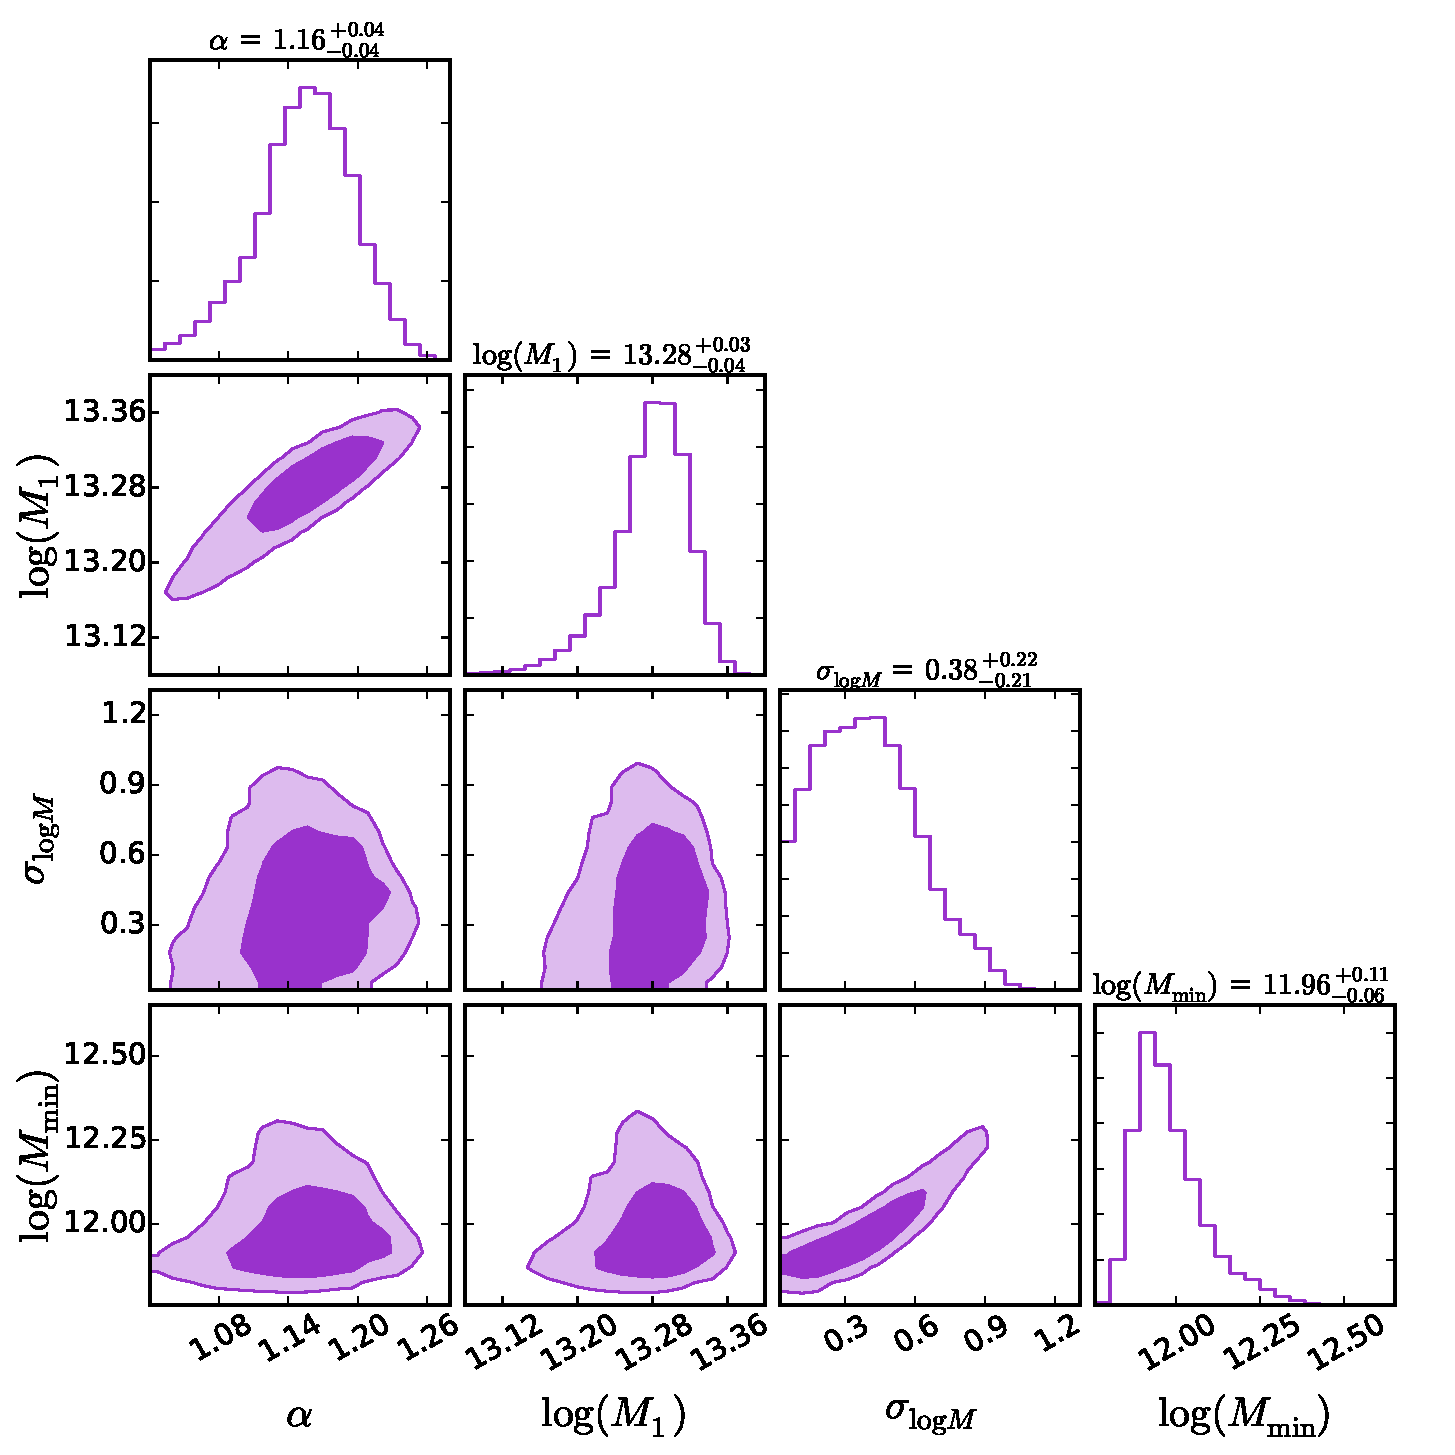
\includegraphics[width=15.0cm]{Mr20_covar_triangle_1.pdf}
\caption{
Two-dimensional marginalized constraints on HOD parameters inferred from 
standard HOD fits to $\wprp(\rp)$ data for the $M_r<-20$ sample. The HOD parameter 
$\log (M_0)$ is extremely poorly constrained by the $\wprp(\rp)$ data and has been 
omitted. The inner contours contain $68\%$ of the posterior probability while the 
outer contours contain $95\%$ of the probability. The panels along the diagonal 
show the one-dimensional, marginalized posteriors on each of these parameters. 
The values above each panel on the diagonal show the 
median value for the parameter in our chains along with the 
16$^{\rm th}$ and 84$^{\rm th}$ percentiles. 
}
\label{fig:Mr20triangle}
\end{center}
\end{figure*}
%----------------------------------------------------------------------------------------------------------------------------------

The inferred parameters from our standard analyses differ in several ways from the \citet{zehavi_etal11} 
analysis. Firstly, in our re-analysis of the projected clustering data, we generally find all mass scales to 
be slightly higher than in the work of \citet{zehavi_etal11}. This difference is largely due to the slightly 
different cosmologies adopted in this work. The most important difference 
are in the values of $\Omega_{\rm M}$, and $\sigma_8$.  
\citet{zehavi_etal11} assumed $\Omega_{\rm M}=0.25$ and $\sigma_8=0.8$, 
whereas in the present work, we use the BolshoiP simulation in which $\Omega_{\rm M}=0.307$ and $\sigma_8=0.82$. 
Slightly larger mass scales are necessary in an analysis with higher $\Omega_{\rm M}$ and $\sigma_8$ in order 
to maintain galaxy number densities with larger halo number densities.

 
%-------------------------------------------------------------------------------------------------------------------------------------------------
\begin{table*}
{\renewcommand{\arraystretch}{1.3}
\renewcommand{\tabcolsep}{0.2cm}
\begin{tabular}{l l c c c c c c c}
\hline 
\hline
Sample $M_r$ &  Authors & $\log (M_{\rm min})$ & $\sigma_{\log M}$ & $ \log (M_1)$ & $\alpha$ & $A_{\rm cen}$ & $A_{\rm sat}$ & $\chi^2/\mathrm{DoF}$\\ 
\hline
$-21$ & Zehavi+11 & $12.78 \pm 0.10$ & $0.68 \pm 0.15$ & $13.80 \pm 0.03$ & $1.15 \pm 0.06$ & $--$ & $--$ & 3.1\\
$-21$ & Zentner+16 & $12.92^{+0.07}_{-0.11}$ & $0.74^{+0.09}_{-0.16}$ & $13.93^{+0.04}_{-0.05}$ & $1.23^{+0.10}_{-0.12}$ & $--$ & $--$ & 1.59\\
$-21$ & Zentner+16 & $12.83^{+0.11}_{-0.09}$ & $0.60^{+0.15}_{-0.17}$ & $13.93^{+0.05}_{-0.08}$ & $1.16^{+0.12}_{-0.14}$ & $0.29^{+0.44}_{-0.35}$ & $0.08^{+0.49}_{-0.36}$ & 1.34 \vspace*{5pt}\\
%
$-20.5$ & Zehavi+11 & $12.14 \pm 0.03$ & $0.17 \pm 0.15$ & $13.44 \pm 0.03$ & $1.15 \pm 0.03$ & $--$ & $--$ & 2.7\\
$-20.5$ & Zentner+16 & $12.25^{+0.07}_{-0.03}$ & $0.23^{+0.17}_{-0.15}$ & $13.59^{+0.02}_{-0.02}$ & $1.20^{+0.04}_{-0.04}$ & $--$ & $--$ & 1.90\\
$-20.5$ & Zentner+16 & $12.32^{+0.13}_{-0.08}$ & $0.45^{+0.21}_{-0.25}$ & $13.59^{+0.04}_{-0.04}$ & $1.14^{+0.05}_{-0.06}$ & $>0.08 (90\%)$ & $0.22^{+0.40}_{-0.31}$ & 1.40 \vspace*{5pt}\\
%
$-20$ & Zehavi+11 & $11.83 \pm 0.03$ & $0.25 \pm 0.11$ & $13.08 \pm 0.03$ & $1.00 \pm 0.05$ & $--$ & $--$ & 2.1\\
$-20$ & Zentner+16 & $11.95^{+0.11}_{-0.6}$ & $0.37^{+0.23}_{-0.21}$ & $13.28^{+0.03}_{-0.04}$ & $1.16^{+0.04}_{-0.04}$ & $--$ & $--$ & 2.19\\
$-20$ & Zentner+16 & $12.23^{+0.33}_{-0.21}$ & $0.84^{+0.37}_{-0.31}$ & $13.20^{+0.06}_{-0.08}$ & $1.05^{+0.06}_{-0.08}$ & $ >0.28 (99\%) $ & $0.01^{+0.32}_{-0.26}$ & 1.16 \vspace*{5pt}\\
%$-20^d$ & Zentner+16 & $11.91^{+0.10}_{-0.03}$ & $0.26^{+0.25}_{-0.17}$ & $13.34^{+0.04}_{-0.05}$ & $1.25^{+0.05}_{-0.06}$ & $--$ & $--$ & 0.70 \\
%$-20^d$ & Zentner+16 & $12.00^{+0.29}_{-0.12}$ & $0.51^{+0.42}_{-0.32}$ & $13.31^{+0.06}_{-0.09}$ & $1.17^{+0.08}_{-0.09}$ & $0.76^{+0.18}_{-0.43}$ & $0.11^{+0.37}_{-0.34}$ & 0.30\vspace*{3pt}\\
$-19.5$ & Zehavi+11 & $11.57 \pm 0.04$ & $0.17 \pm 0.13$ & $12.87 \pm 0.03$ & $0.99 \pm 0.04$ & $--$ & $--$ & 1.00 \\
$-19.5$ & Zentner+16 & $11.76^{+0.33}_{-0.11}$ & $0.51^{+0.51}_{-0.29}$ & $13.05^{+0.04}_{-0.08}$ & $1.12^{+0.04}_{-0.07}$ & $--$ & $--$ & 1.24\\
$-19.5$ & Zentner+16 & $11.80^{+0.36}_{-0.16}$ & $0.63^{+0.53}_{-0.37}$ & $13.04^{+0.09}_{-0.12}$ & $1.06^{+0.07}_{-0.10}$ & $>-0.01 (84\%)$ & $>-0.16 (84\%)$ & 0.69 \vspace*{5pt}\\
%
$-19$ & Zehavi+11 & $11.45 \pm 0.04$ & $0.19 \pm 0.13$ & $12.64 \pm 0.04$ & $1.02 \pm 0.02$ & $--$ & $--$ & 1.8 \\
$-19$ & Zentner+16 & $11.72^{+0.33}_{-0.19}$ & $0.69^{+0.52}_{-0.46}$ & $12.78^{+0.04}_{-0.04}$ & $1.03^{+0.04}_{-0.04}$ & $--$ & $--$ & 2.77\\
$-19$ & Zentner+16 & $11.62^{+0.33}_{-0.13}$ & $0.53^{+0.57}_{-0.35}$ & $12.83^{+0.06}_{-0.07}$ & $1.02^{+0.04}_{-0.04}$ & $0.35^{+0.45}_{-0.66}$ & $>0.02 (84\%)$ & 2.01\\
%$-19^d$ & Zentner+16 & $11.87^{+0.17}_{-0.27}$ & $1.10^{+0.30}_{-0.52}$ & $12.84^{+0.17}_{-0.23}$ & $1.11^{+0.15}_{-0.15}$ & $--$ & $--$ & 2.30 \\
%$-19^d$ & Zentner+16 & $11.75^{+0.24}_{-0.27}$ & $0.94^{+0.41}_{-0.55}$ & $12.99^{+0.14}_{-0.18}$ & $1.17^{+0.14}_{-0.14}$ & $-0.17^{+0.50}_{-0.47}$ & $$ & 1.70\\
\hline
\end{tabular}
\medskip
\caption{
Results of standard HOD fits to SDSS DR7 $w_{\rm p}(r_{\rm p})$ as well as 
fits using a parameterized model of assembly bias. 
Assembly bias is quantified by the parameters $A_{\rm cen}$ ($A_{\rm sat}$) for central (satellite) galaxies. The secondary 
property that we assume to determine the galaxy HOD is halo formation time. $A_{\rm cen,sat}=0$ means that there is no 
assembly bias while $A_{\rm cen,sat}=1$ ($A_{\rm cen,sat}=-1$) means that halo formation time is maximally 
correlated (anticorrelated) with halo formation time. Thus the parameters range over $-1 \le A_{\rm cen,sat} \le 1$. 
If the constraints on $A_{\rm cen}$ and $A_{\rm sat}$ are unspecified, then the model used to interpret the data 
does not include assembly bias. In our analyses, quoted parameter values with errors correspond to the median 
value of the parameter and the 16$^{\rm th}$ and 84$^{\rm th}$ percentiles. In cases for which the posterior 
is monotonic within the physical parameter space, we show one-sided percentiles.
}
}
 \label{table:parameters}
\end{table*}
%---------------------------------------------------------------------------------------------------------------------------------


%----------------------------------------------------------------------------------------------------------------------------------
\begin{figure*}
\begin{center}
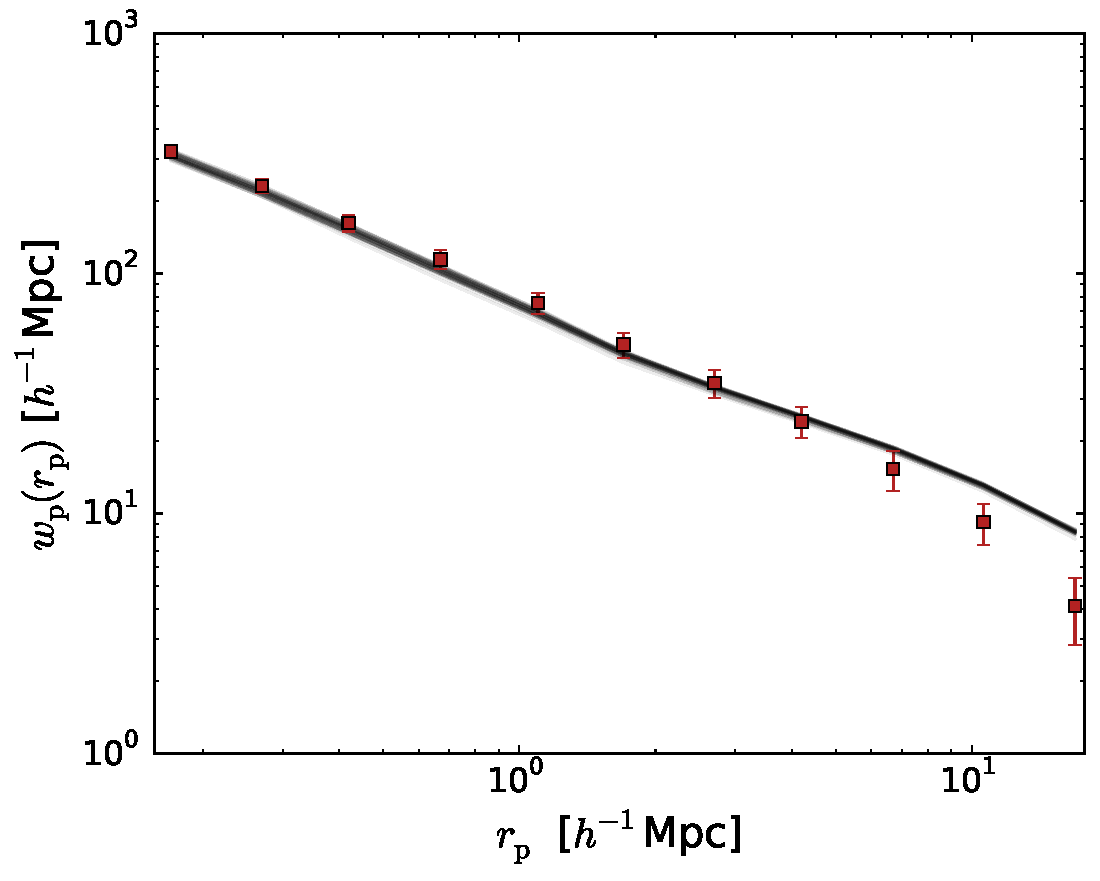
\includegraphics[width=8.3cm]{Mr19samples.pdf}
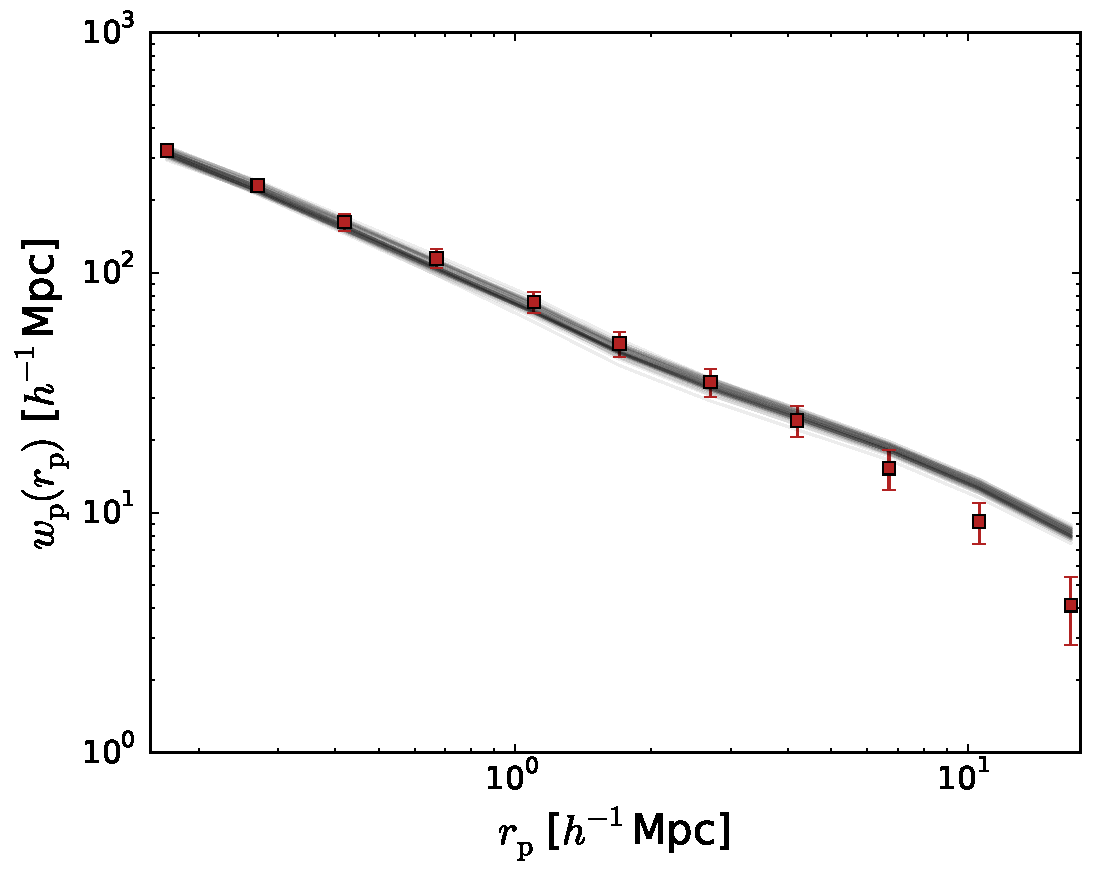
\includegraphics[width=8.3cm]{Mr19ABsamples.pdf}
\caption{
{\bf Left:} The $M_r<-19$ threshold sample projected correlation function with diagonal elements of 
covariance (points with errorbars). The grey lines are 25 randomly-selected HOD models that yield 
$\Delta \chi^2 <1$ compared to the best-fitting model. {\bf Right:} Same as the left panel but using a 
fit to a Decorated HOD model that contain parameters to describe the strength of assembly bias.
}
\label{fig:Mr19samples}
\end{center}
\end{figure*}
%---------------------------------------------------------------------------------------------------------------------------------


%---------------------------------------------------------------------------------------------------------------------------------
\begin{figure*}
\begin{center}
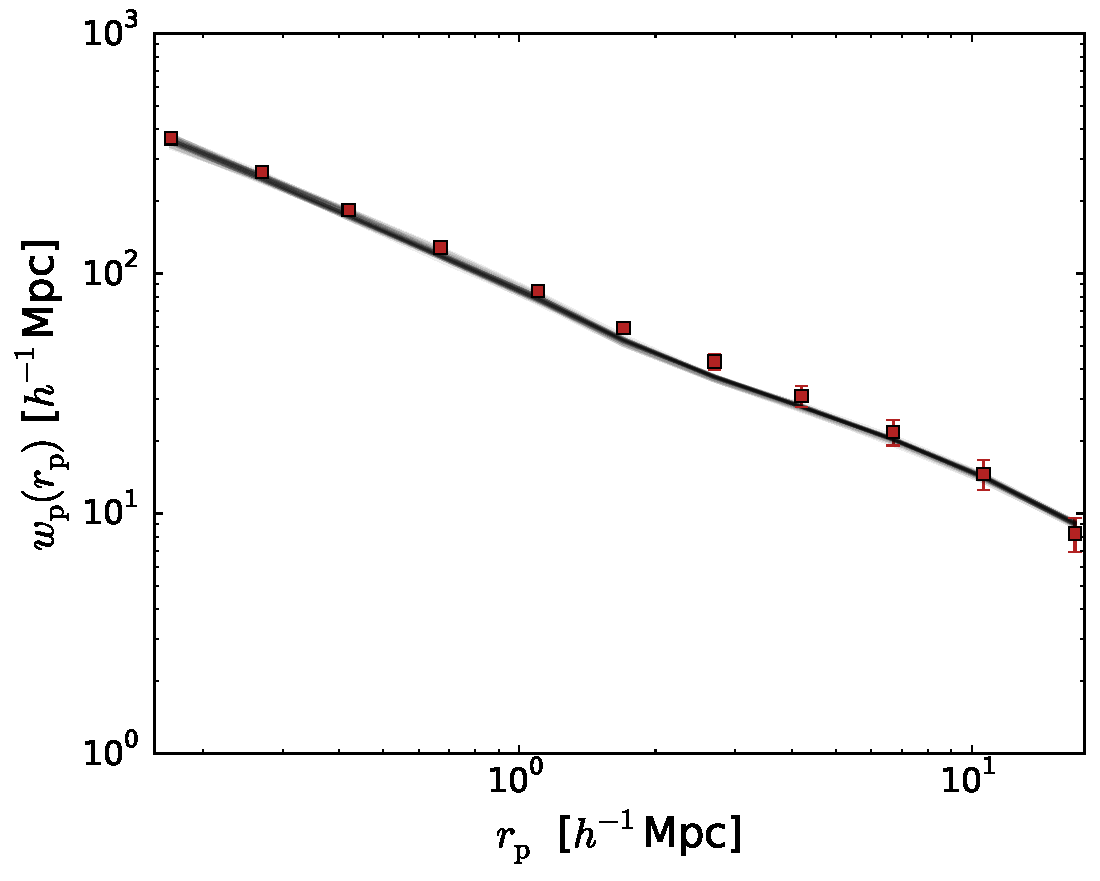
\includegraphics[width=8.3cm]{Mr20samples.pdf}
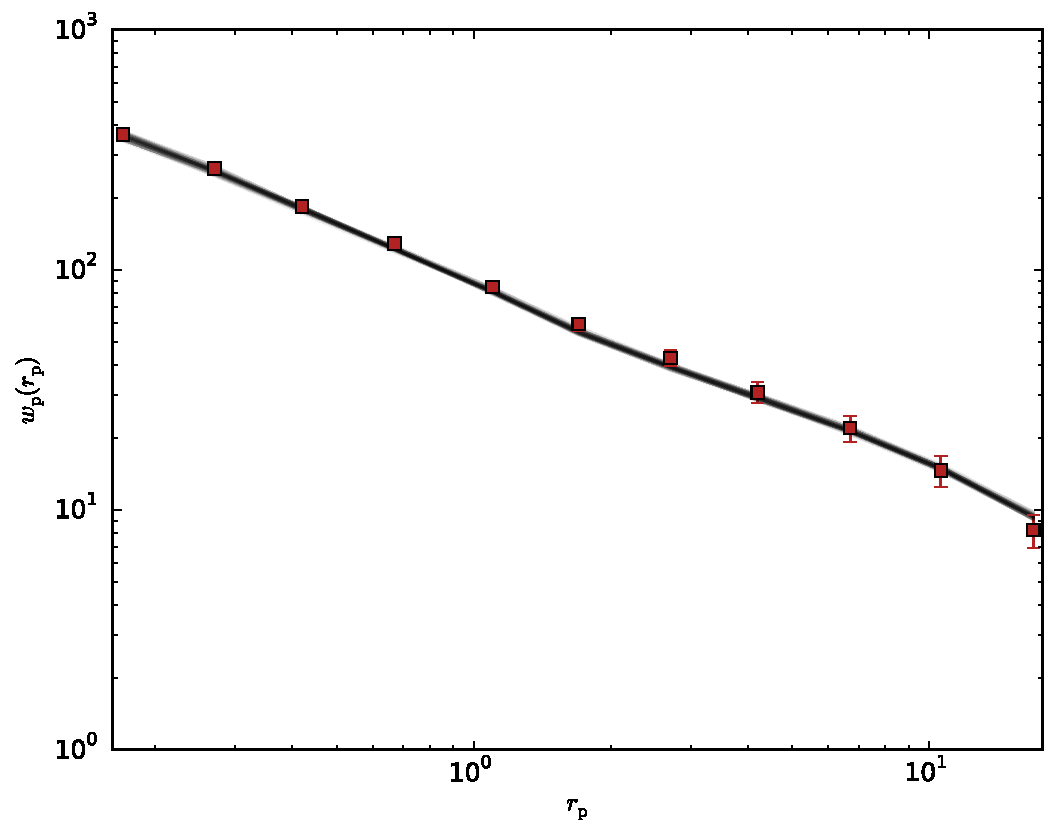
\includegraphics[width=8.3cm]{Mr20ABsamples.pdf}
\caption{
The same as Figure~\ref{fig:Mr19samples}, but for the $M_r<-20$ threshold sample.
}
\label{fig:Mr20samples}
\end{center}
\end{figure*}
%---------------------------------------------------------------------------------------------------------------------------------


%---------------------------------------------------------------------------------------------------------------------------------
\begin{figure*}
\begin{center}
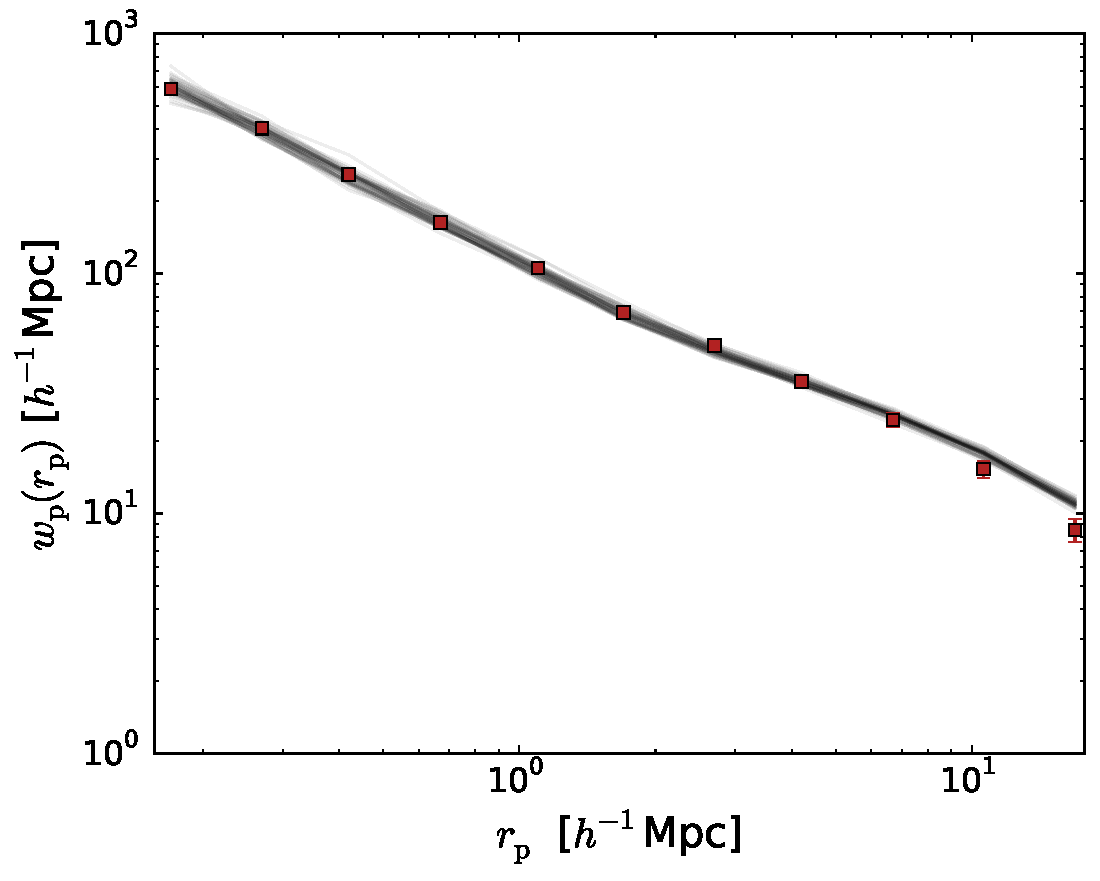
\includegraphics[width=8.3cm]{Mr21samples.pdf}
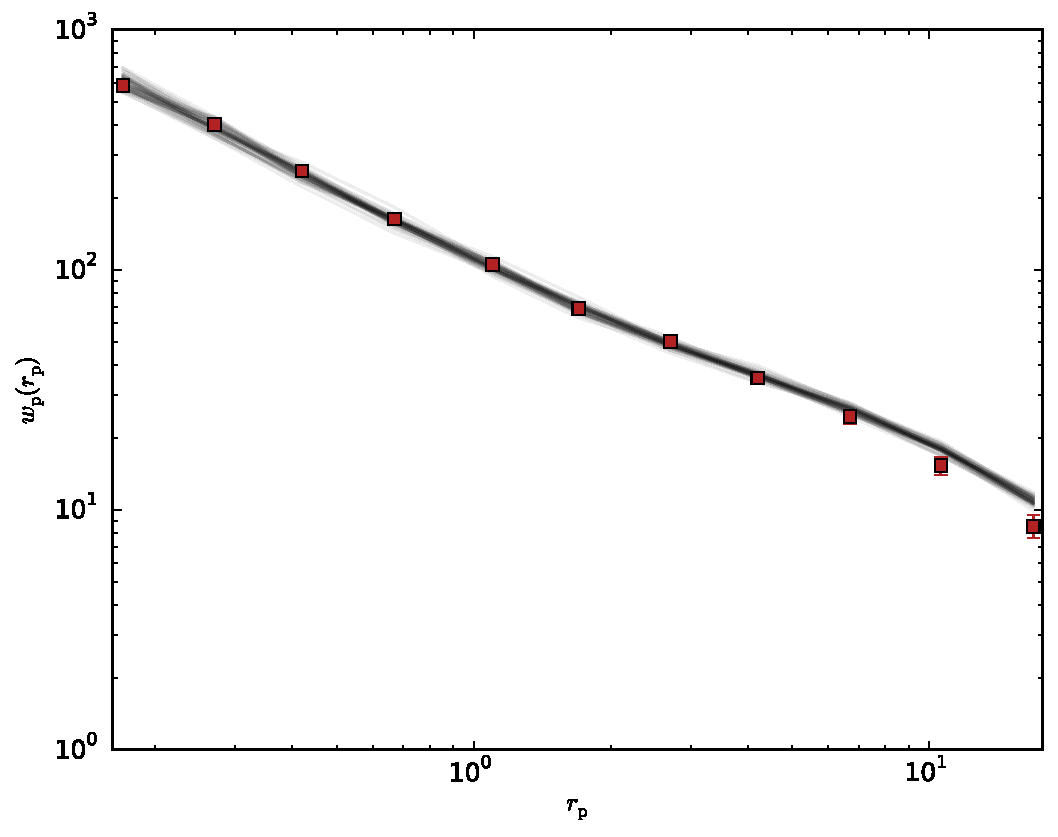
\includegraphics[width=8.3cm]{Mr21ABsamples.pdf}
\caption{
The same as Figure~\ref{fig:Mr19samples}, but for the $M_r<-21$ threshold sample.
}
\label{fig:Mr21samples}
\end{center}
\end{figure*}
%---------------------------------------------------------------------------------------------------------------------------------


A second noteworthy difference between the present work and that of \citet{zehavi_etal11} is that we 
find many parameters to be notably more poorly constrained. At the lower luminosity thresholds, for example, 
we constrain $\log (M_{\rm min})$ and $\sigma_{\log M}$ with several times lower precision than 
\citet{zehavi_etal11}. We do not show our constraints on $\log (M_0)$ as they are very poor in all cases, 
with 1-sigma constraints on the order of $\pm \ge 1$~dex for nearly all samples. In several cases, the constraint on 
$\log (M_0)$ is determined by the prior given in Table~\ref{table:priors}. This is in stark contrast to several of the 
results of \citet{zehavi_etal11}. For example, for the threshold sample with $M_r < -19.5$ ($M_r < -20.5$), 
\citet{zehavi_etal11} quote $\log (M_0) = 12.23 \pm 0.17$ ($12.35 \pm 0.24$), whereas we infer 
$\log (M_0) = 11.38^{+0.95}_{-1.57}$ ($11.19^{+0.89}_{-1.39}$). Examining the form of Eq.~(\ref{eq:nsat}), 
it is sensible that the parameter $\log (M_0)$ should be unconstrained at the lower end, because the 
value of $M_0$ does not alter the predicted satellite number once $M_0 \ll M_1$. Therefore, it seems likely 
that the tighter constraints quoted by \citet{zehavi_etal11} must be an error. 

We have confirmed with a subset of the authors of \citet{zehavi_etal11} 
that the number of MCMC samples they included in their analysis was 
insufficient in a number of cases and that this can lead to a significant underestimation of the uncertainties 
on the inferred parameters, especially $\log (M_{\rm min})$ and $\sigma_{\log M}$ 
(Z. Zheng \& I. Zehavi, Private Communication). The analysis of \citet{zehavi_etal11} 
used $10^4$ samples, whereas we find several $\times 10^6$ samples are often necessary for convergence. 
Additionally, we have recreated qualitatively similar behavior by considering only small subsets of all of our 
full MCMC chains. Consequently, insufficient sampling of the posterior seems to be the likely resolution 
of the discrepancies between our work and that of \citet{zehavi_etal11}.

Two degeneracies are manifest in Fig.~\ref{fig:Mr20triangle} that are common to all of our 
analyses. The parameters $\log (M_1)$ and $\alpha$ are degenerate with each other and positively 
correlated. The parameter $M_1$ is the mass scale at which a halo has one satellite on 
average and $\alpha$ is the power-law index describing the dependence of average satellite 
number on halo mass. Increasing $M_1$ decreases the number of satellites in large halos 
by placing satellites preferentially in halos of larger mass. An increase in $\alpha$ can partly 
compensate for an increase in $M_1$ by increasing the rate at which average satellite number 
grows with halo mass, leading to a larger number of satellites in high-mass halos. 

As is evident in Figure~\ref{fig:Mr20triangle}, $\log (M_{\rm min})$ and $\sigma_{\log M}$ 
share a relatively narrow degeneracy as well. This degeneracy is largely induced by the 
measured number density of the sample. Increasing $\log (M_{\rm min})$ decreases galaxy 
number density, but this can be compensated by an increase in $\sigma_{\log M}$, which 
places galaxies in a fraction of the considerably more numerous halos with masses less 
than $M_{\rm min}$. The consequence is that $\log (M_{\rm min})$ and $\sigma_{\log M}$ are 
degenerate with each other such that most of the posterior probability lies in a narrow band 
along which $\log (M_{\rm min})$ and $\sigma_{\log M}$ are positively correlated, as shown in 
Fig.~\ref{fig:Mr20triangle}. In the following plots, we suppress the parameter $\sigma_{\log M}$,  
in order to increase the clarity of the plots, because the viable range of $\sigma_{\log M}$ is 
determined by this simple degeneracy with $\log (M_{\rm min})$. 

The results of this subsection demonstrate that we achieve reasonable fits to projected galaxy clustering 
data using direct HOD population of a high-resolution numerical simulation of structure formation. These results 
also update and supersede existing constraints in the literature in at least three respects. First, we work within the 
best-fit Planck cosmology. Second, we perform our parameter inference analysis using direct population of halos 
identified in a numerical simulation of cosmological structure formation (BolshioP). This greatly mitigates modeling 
uncertainties associated with nonlinear density field evolution, scale-dependent halo bias, halo exclusion, 
or other effects that have been difficult to incorporate into analytical halo models with high precision. Third, 
we have explored the posteriors of the parameters with significantly more samples (roughly two orders of magnitude), 
thereby mitigating errors on inferred parameters and their errors induced by insufficient sampling of the 
posterior.

%-------------------------
\subsection{Analysis with Decorated HOD}
\label{subsection:ab}
%-------------------------

We turn now to a discussion of our parameter inference analysis of projected galaxy clustering 
in Decorated HOD models that include a treatment of galaxy assembly bias. In this work, 
we consider only the simplest model of galaxy assembly bias, introducing only two new 
parameters, $A_{\rm cen}$ and $A_{\rm sat}$, that describe the strength of central galaxy 
and satellite galaxy assembly bias respectively. These parameters are limited to values 
of $-1 \le A_{\rm cen,sat} \le 1$, and $A_{\rm cen,sat}=0$ when there is no galaxy assembly bias. 
In this work, we use halo concentration as our secondary halo property, so $A_{\rm cen,sat}=1$ 
($A_{\rm cen,sat}=-1$) means that the mean number of galaxies per halo is maximally 
correlated (anti-correlated) with halo concentration. The model and its implementation 
in {\tt halotools} is discussed further in Section~\ref{subsection:decorated} above and 
in \citet{hearin_etal16}.

Examples of our fits are given in the right-hand panels of Figure~\ref{fig:Mr19samples}, 
Figure~\ref{fig:Mr20samples}, and Figure~\ref{fig:Mr21samples}. The general trend that 
can be gleaned from these figures is that introducing assembly bias improves the ability 
of the predicted two-point functions to match the measured two-point functions across the 
transition form the one-halo (highly nonlinear) to two-halo (nearly linear) regimes near $\rp \sim 2\, h^{-1}{\mathrm{Mpc}}$. 
This is most apparent for the $M_r < -20$ threshold sample shown in Fig.~\ref{fig:Mr20samples}. 
Visually, these differences appear to be small; however, Table~\ref{table:parameters} shows that 
they are statistically important.

The one-dimensional marginalized constraints on all parameters from these analyses 
are given in the lowest row of each luminosity threshold grouping in Table~\ref{table:parameters}. 
In cases where the posterior on a parameter is monotonic within the physical parameter 
range, we quote an upper or lower limit on the parameter. One- and two-dimensional 
visualizations of the posteriors from our analysis are shown in Figure~\ref{fig:Mr19ABtriangle}, 
Figure~\ref{fig:Mr20ABtriangle}, and Figure~\ref{fig:Mr21ABtriangle}. 


%------------------------------------------------------------------------------------------------
\begin{figure*}
\begin{center}
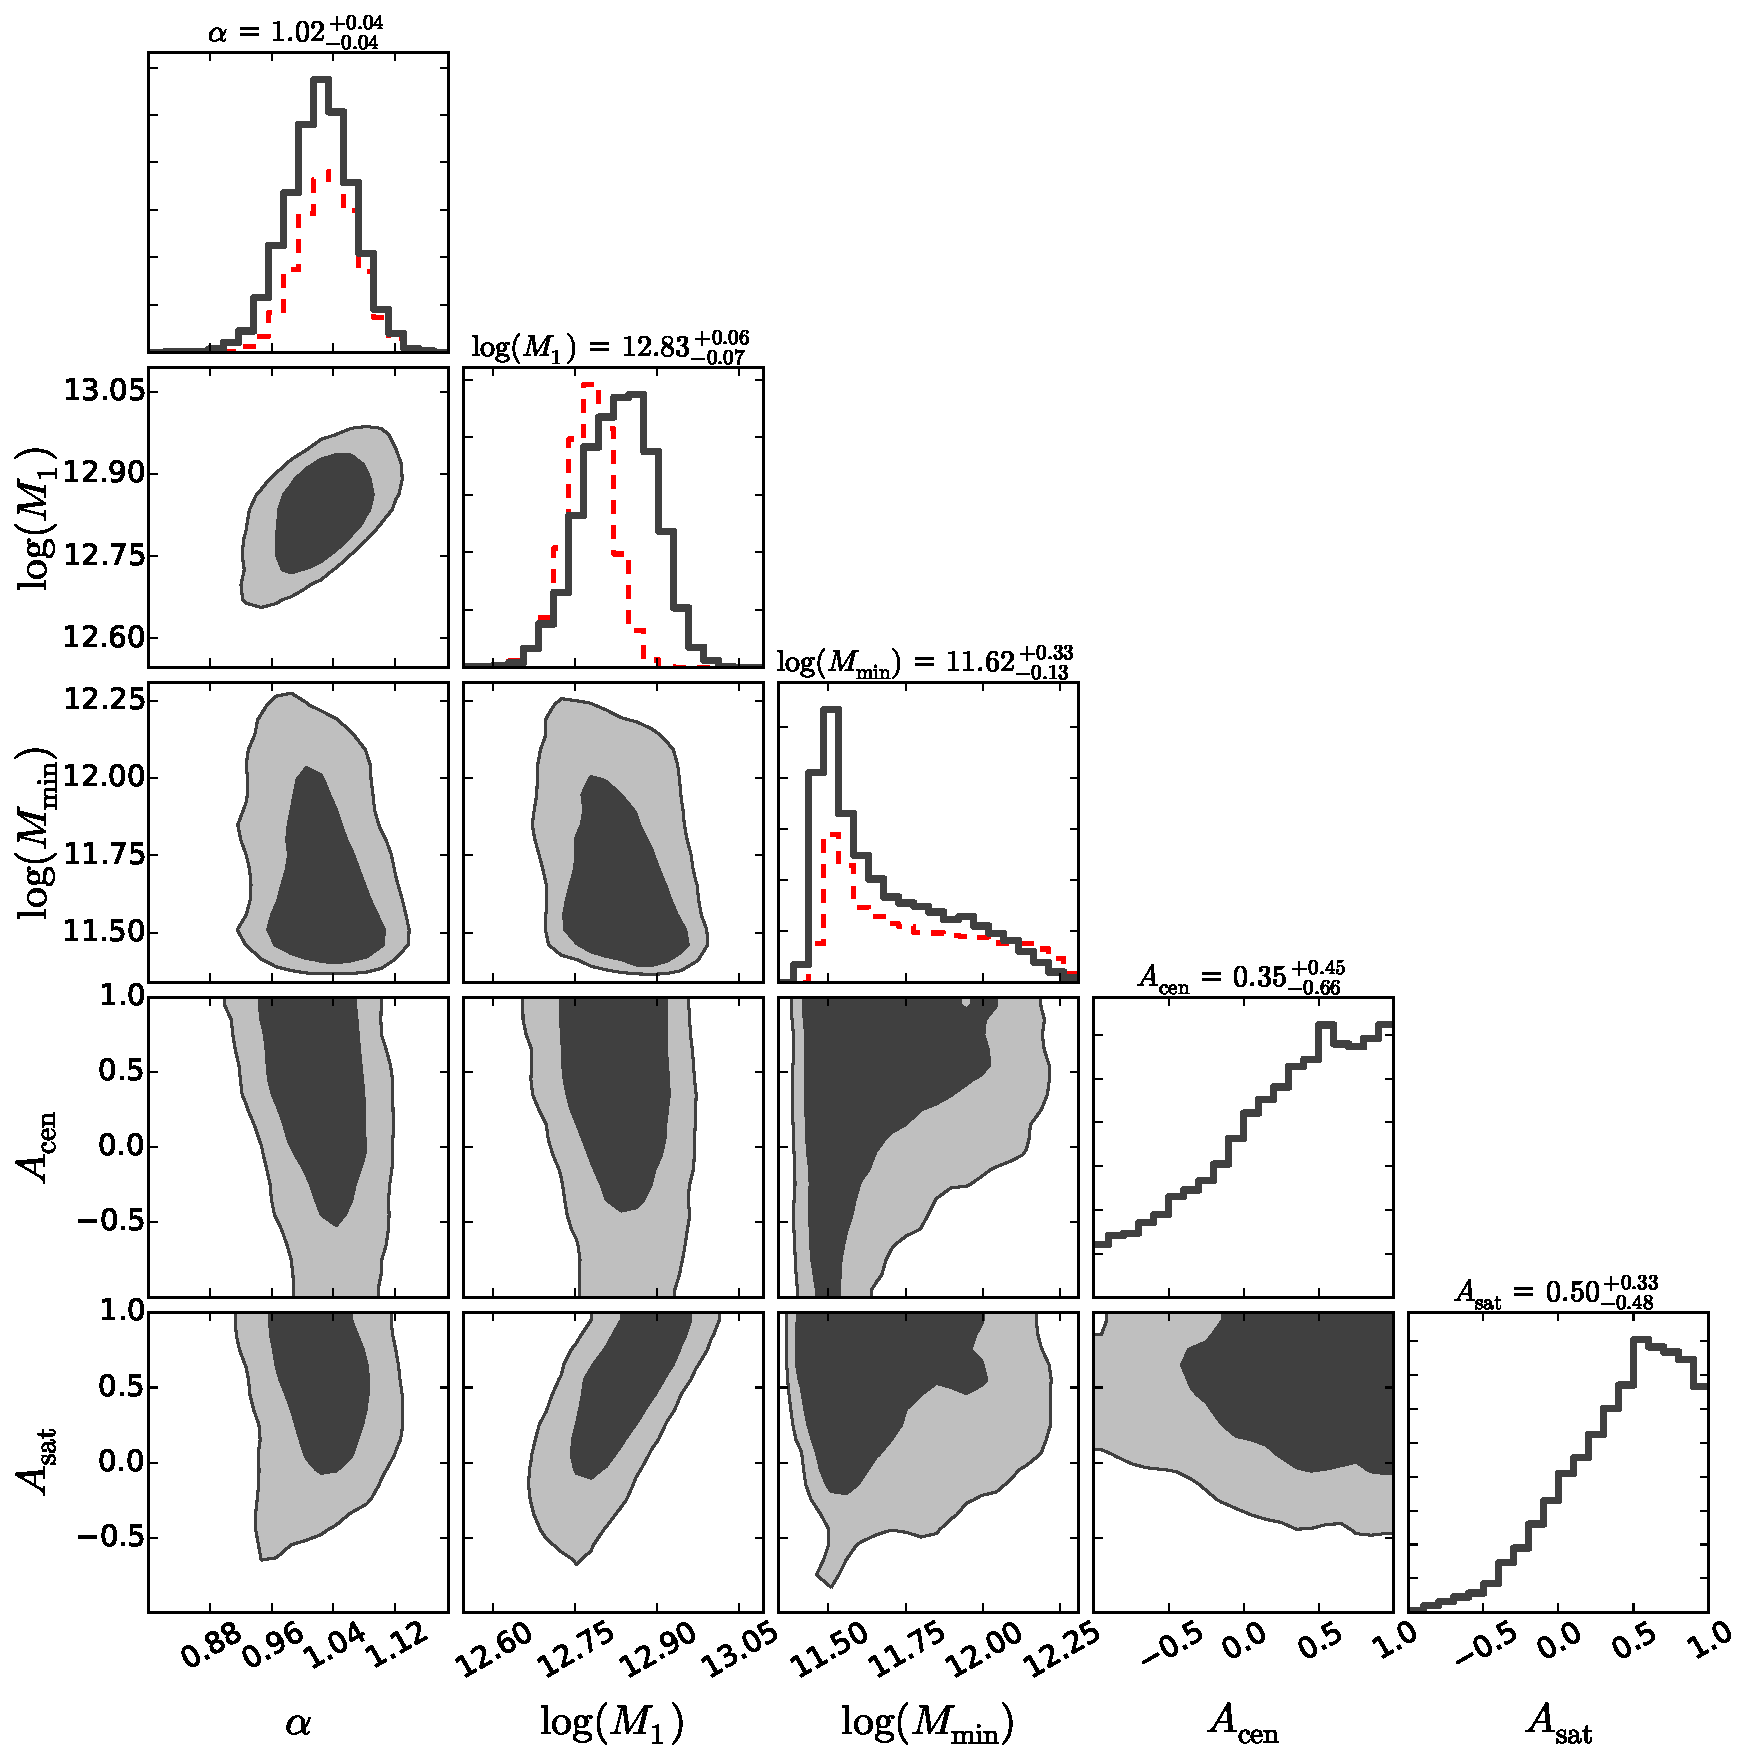
\includegraphics[width=15.0cm]{Mr19ABTri.pdf}
\caption{
Two-dimensional marginalized constraints on decorated HOD parameters inferred from fits 
to $\wprp(\rp)$ data for the $M_r<-19$ sample. The contours and histograms along the diagonal 
panels are as in Fig.~\ref{fig:Mr20triangle}. The decorated HOD models include a 
two-parameter model for assembly bias. The HOD parameter $\log (M_0)$ is extremely 
poorly constrained by the data and has been suppressed for clarity. Likewise, as in 
Fig.~\ref{fig:Mr20triangle}, $\sigma_{\log M}$ and $\log (M_{\rm min})$ share a 
narrow degeneracy, so we have suppressed $\sigma_{\log M}$ in order to make 
constraints on other parameters more easily visible.
}
\label{fig:Mr19ABtriangle}
\end{center}
\end{figure*}
%----------------------------------------------------------------------------------------------


%---------------------------------------------------------------------------------------------------
\begin{figure*}
\begin{center}
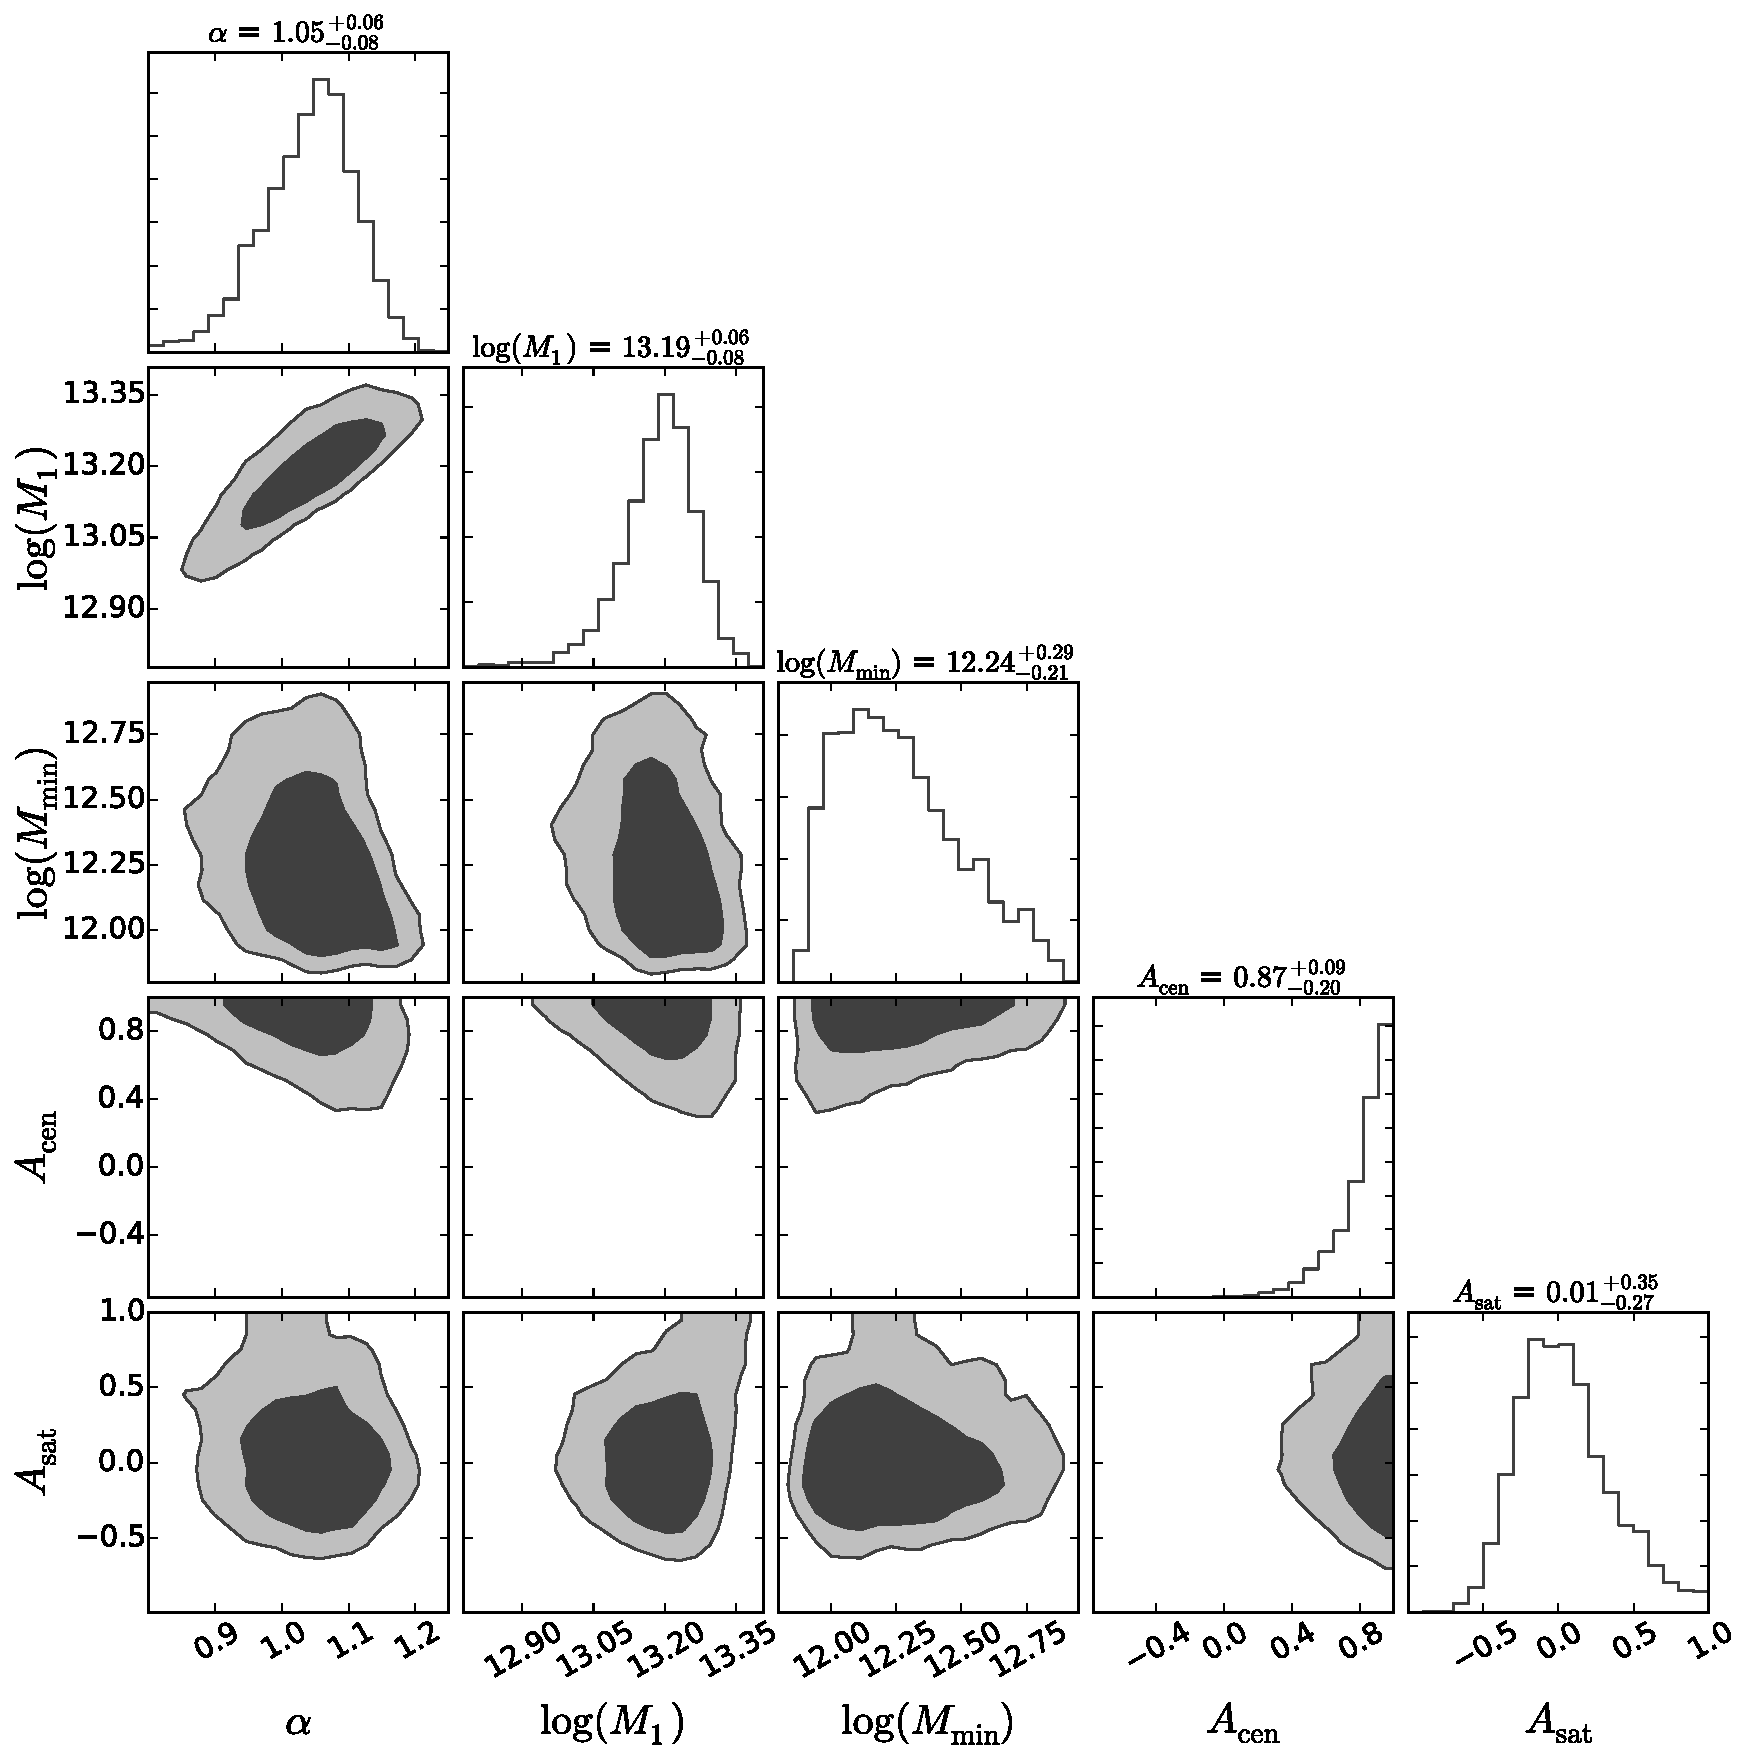
\includegraphics[width=15.0cm]{Mr20ABTri.pdf}
\caption{
The same as Figure~\ref{fig:Mr19ABtriangle}, but for the $M_r<-20$ sample.
}
\label{fig:Mr20ABtriangle}
\end{center}
\end{figure*}
%---------------------------------------------------------------------------------------------------

%=-------------------------------------------------------------------------------------------------
\begin{figure*}
\begin{center}
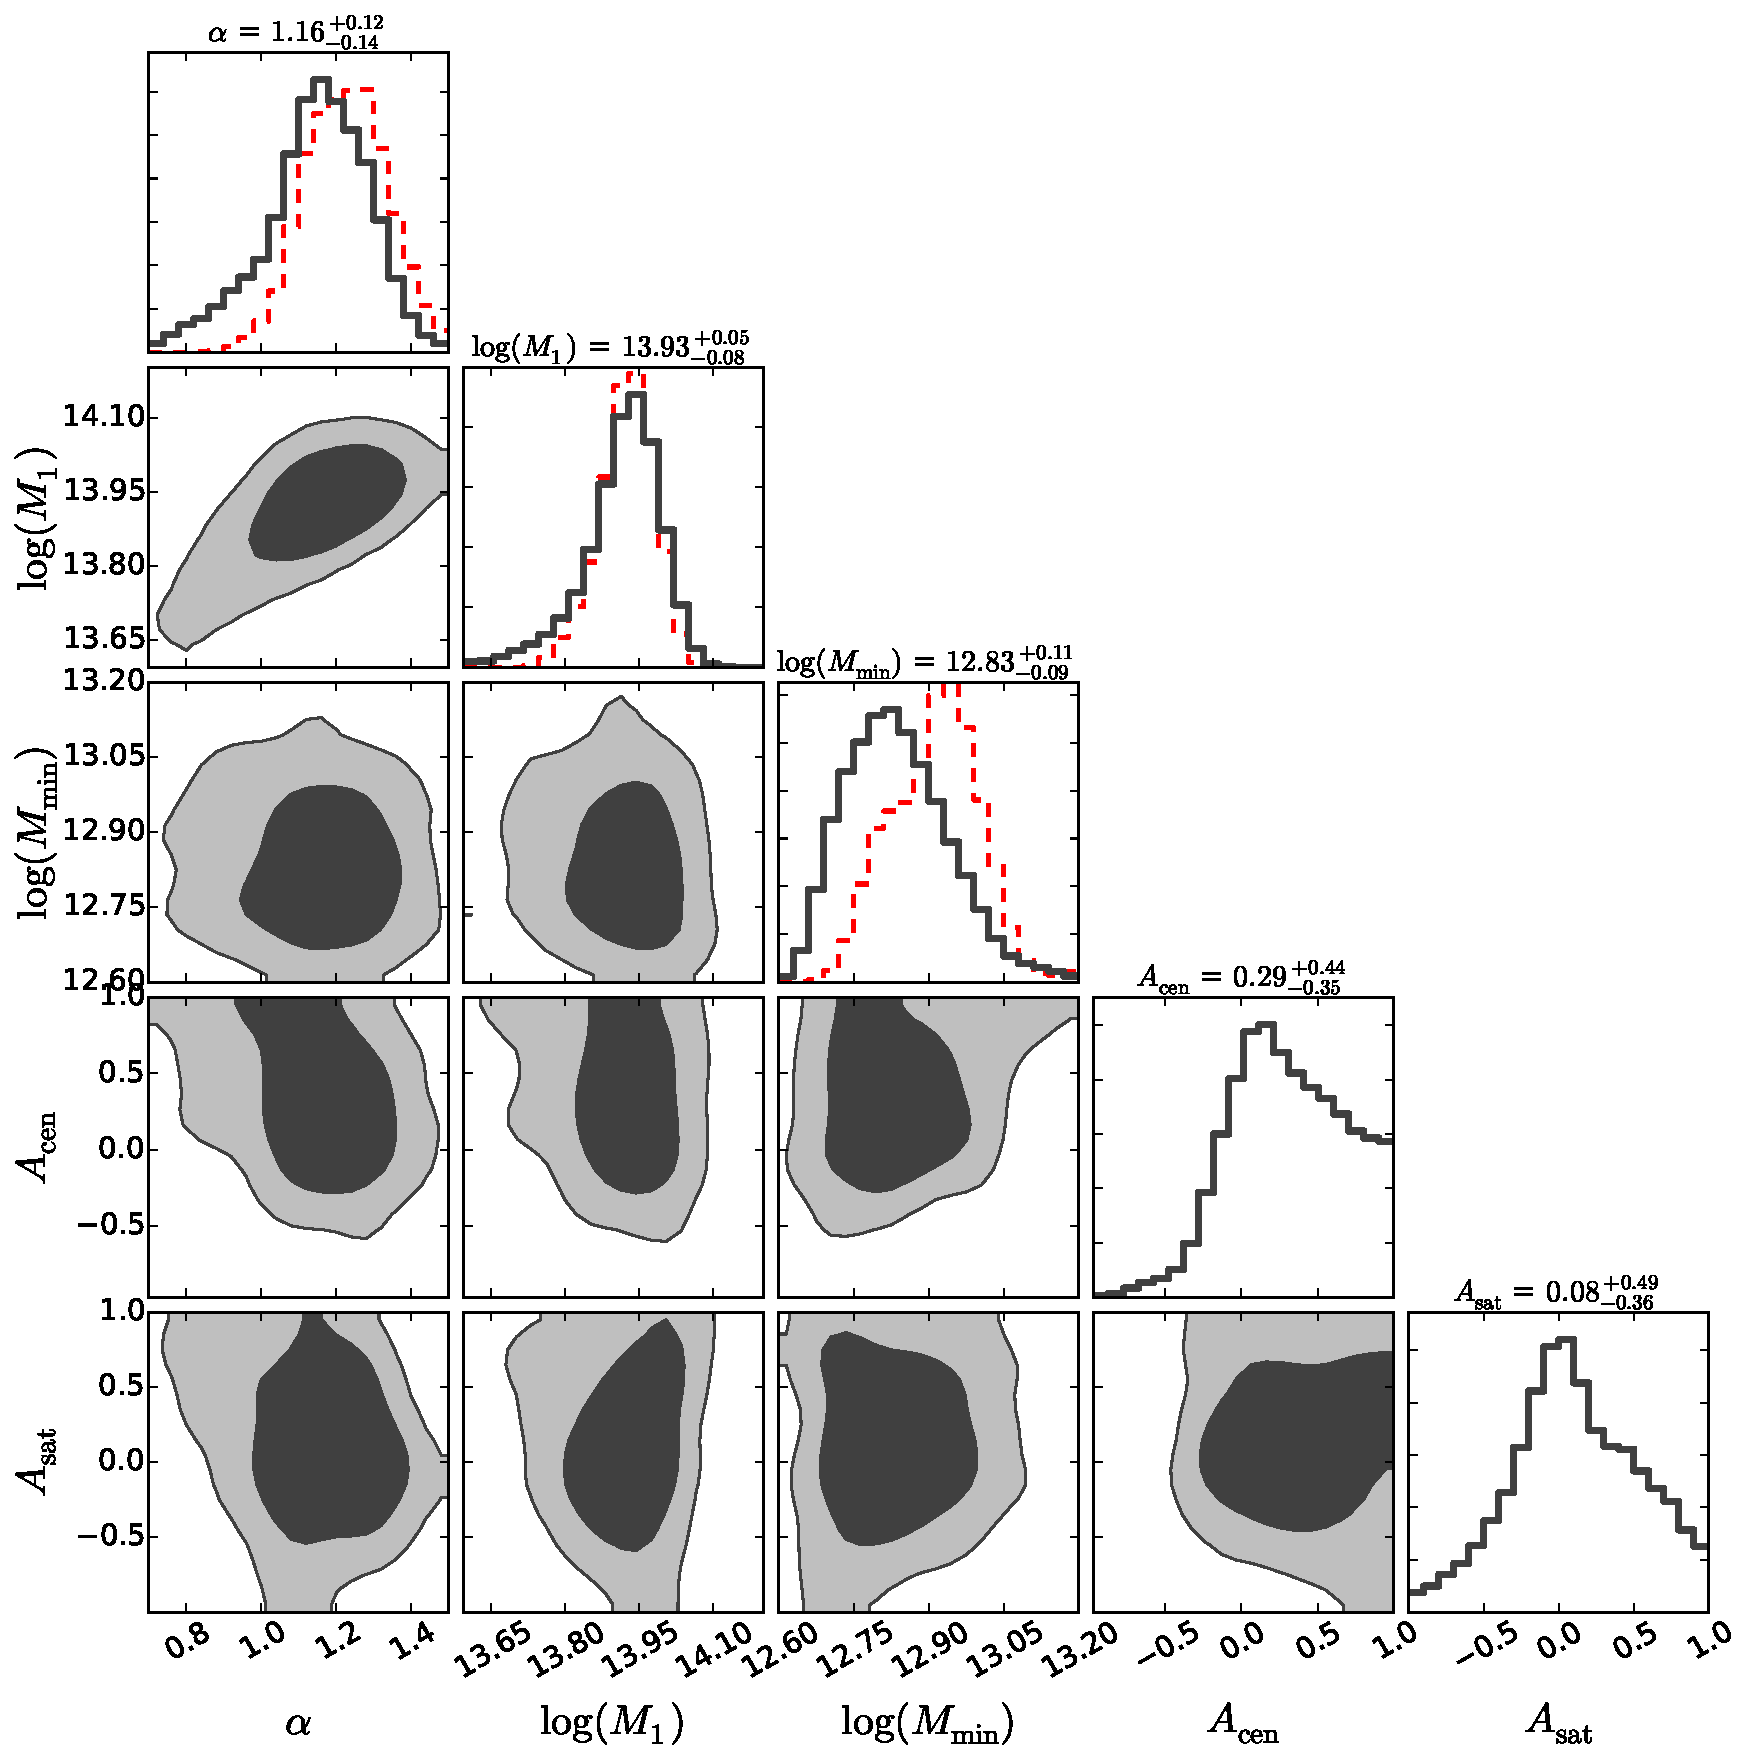
\includegraphics[width=15.0cm]{Mr21ABTri.pdf}
\caption{
The same as Figure~\ref{fig:Mr19ABtriangle}, but for the $M_r<-21$ sample.
}
\label{fig:Mr21ABtriangle}
\end{center}
\end{figure*}
%----------------------------------------------------------------------------------------------------


Table~\ref{table:parameters} and Figures~\ref{fig:Mr19ABtriangle}-\ref{fig:Mr21triangle} 
all make several simple, generic points. Introducing additional parameter 
freedom associated with galaxy assembly bias generally increases the viable parameter 
space, even for the subset of standard HOD parameters. This is exactly what is 
expected from the introduction of additional parameter freedom. 

Focusing attention on the parameters describing galaxy assembly bias, it is 
evident that these parameters are often quite poorly constrained by galaxy 
clustering data. This implies that galaxy clustering of the precision of SDSS DR7 
measurements cannot rule out, or strongly restrict galaxy assembly bias in most 
cases. 

Beyond those generic conclusions, a few specific cases of worthy of further examination. 
Consider the $M_r < -20$ sample. The inferred value of $A_{\rm cen} > 0.28$ at 99\% 
confidence. In this case the data strongly prefer $A_{\rm cen} > 0$ and thus strongly prefer 
galaxies to reside in halos of larger concentration at fixed halo mass. 

Changes in Bayesian Information Criterion, for inclusion in some sort of table. Strong evidence 
is usually considered to be a difference $>5$.

Delta BIC 19: 4.37

Delta BIC 19.5: 0.26

Delta BIC 20: 4.56

Delta BIC 20.5: 1.33

Delta BIC 21: -0.54

%------------------------------------------------


%------------------------------------------------
\section{Conclusions}
\label{section:conclusions}
%------------------------------------------------




%------------------------------------------------
\bibliography{ms.bib}

%------------------------------------------------
\end{document}
%------------------------------------------------
